\documentclass{article}

\usepackage{iclr2027_conference,times}
\usepackage{amsmath,amssymb,mathtools,amsthm}
\usepackage{booktabs,multirow,array}
\usepackage{graphicx}
\usepackage{subcaption}
\usepackage{xcolor}
\usepackage{microtype}
\usepackage{enumitem}
\usepackage{url}
\usepackage{hyperref}

\definecolor{targetblue}{HTML}{2962A3}
\definecolor{draftorange}{HTML}{E07A2D}
\definecolor{treegreen}{HTML}{238B57}
\definecolor{softgray}{HTML}{666666}
\hypersetup{colorlinks=true,citecolor=targetblue,linkcolor=targetblue,urlcolor=targetblue}

\newtheorem{theorem}{Theorem}
\newtheorem{lemma}{Lemma}
\newtheorem{proposition}{Proposition}
\newtheorem{corollary}{Corollary}
\newtheorem{assumption}{Assumption}
\newcommand{\V}{\mathcal{V}}
\newcommand{\T}{\mathcal{T}}
\newcommand{\C}{\mathcal{C}}
\newcommand{\E}{\mathbb{E}}
\newcommand{\Prb}{\mathbb{P}}
\newcommand{\prefix}{\operatorname{pref}}
\newcommand{\parn}{\operatorname{par}}
\newcommand{\TBV}{\textnormal{\textsc{TBV}}}
\newcommand{\AdaptiveTree}{\textnormal{\textsc{AdaptiveTree}}}
\newcommand{\DFlash}{\textnormal{\textsc{DFlash}}}
\newcommand{\DDTree}{\textnormal{\textsc{DDTree}}}
\newcommand{\method}{\textnormal{\textsc{AdaptiveTree--TBV}}}
% Central switchboard for result values.  Keep these blank until the complete,
% audited formal matrix has passed.  Fill macros here instead of editing prose.
\newcommand{\BlankResult}{\makebox[2.1em]{\rule{1.7em}{0.35pt}}}
\newcommand{\BlankWide}{\makebox[3.7em]{\rule{3.2em}{0.35pt}}}
\newcommand{\PendingResult}{\textcolor{softgray}{\BlankResult}}
\newcommand{\PendingWide}{\textcolor{softgray}{\BlankWide}}


\title{Adaptive Tree Budgets and Exact Tree-Block Verification\\
for Block-Diffusion Speculative Decoding}

\author{Anonymous authors\\
Paper under double-blind review}

\begin{document}
\maketitle

\begin{abstract}
Block-diffusion drafters expose many plausible future tokens in one forward pass, but a decoding system must decide both \emph{which} candidate prefixes deserve target computation and \emph{how} to sample from the verified tree without changing the target distribution.  We present \method, a protocol-separated system with two components.  At temperature zero, \AdaptiveTree selects a node budget online from nested \DDTree{} prefixes using an acceptance-calibrated, budget-aware latency model.  At positive temperature, \TBV keeps the official \DDTree{} proposal tree and every target probability row fixed, but replaces all-row categorical sampling and host traversal by a single persistent CUDA block that performs inverse-CDF sampling only on reached rows.  We prove that the tree forward produces path-local target conditionals, derive the complete variable-length block law, establish exact target-distribution preservation under history-adaptive trees, and prove equivalence of the parallel chunk scan to global inverse-CDF sampling.  The same-tree result also implies that \TBV{} cannot improve acceptance length over \DDTree; any speed difference must come from execution.  We specify a fail-closed evaluation on Qwen3-4B and Qwen3-8B across reasoning, code, and dialogue tasks.  Quantitative result fields are intentionally blank pending a fresh, audited run.
\end{abstract}

\section{Introduction}

Autoregressive language models sample one token per target-model step.  Speculative decoding amortizes this sequential cost by proposing several future tokens with a cheaper model and verifying them in parallel while preserving the target law \citep{leviathan2023fast,chen2023accelerating}.  Its practical speed is governed by three coupled quantities: draft latency, target verification cost, and the number of tokens committed per verification round.

Block diffusion is an appealing drafter because it predicts all future positions in one pass.  \DFlash{} conditions a lightweight block-diffusion model on target features and verifies one path \citep{chen2026dflash}.  \DDTree{} reuses the same position-wise distributions to construct a high-mass prefix tree, then obtains target logits for all tree nodes with one ancestor-masked forward pass \citep{ringel2026ddtree}.  A larger tree can cover more target continuations, but it also increases tree construction, masked attention, vocabulary projection, sampling, and cache-compaction costs.  Therefore, neither a globally fixed budget nor acceptance length alone determines end-to-end throughput.

This work separates two questions that are easy to conflate.  First, at deterministic decoding temperature $T=0$, how should the tree-node budget adapt to the prompt, context length, and measured device costs?  Second, at stochastic temperature $T>0$, how can the already verified tree be traversed with less control overhead while retaining exactly the same conditional target law?  Figure~\ref{fig:overview} shows the resulting architecture.  The two protocols share the block-diffusion proposal and tree representation, but they are evaluated separately: \AdaptiveTree{} is currently a greedy decoder, whereas \TBV{} is the stochastic verifier.

Our contributions are:
\begin{itemize}[leftmargin=1.25em,itemsep=1pt,topsep=2pt]
    \item a corrected latency-aware tree controller that treats tree construction as a budget-dependent cost, expands the candidate range to 256 nodes, and disables periodic exploration after a one-pass warm-up;
    \item an exact same-tree verifier that uses a persistent CUDA block and a parallel chunk scan to sample only target rows reached by ancestral traversal;
    \item a strict derivation of the emitted block distribution, including adaptive-tree conditioning, multi-round exactness, expected accepted length, tree-attention correctness, and the inverse-CDF kernel; and
    \item a preregistered, failure-closed evaluation in which all model revisions, inputs, backends, temperatures, method positions, scorers, and same-tree witnesses are audited before any speed claim is released.
\end{itemize}

\begin{figure}[t]
    \centering
    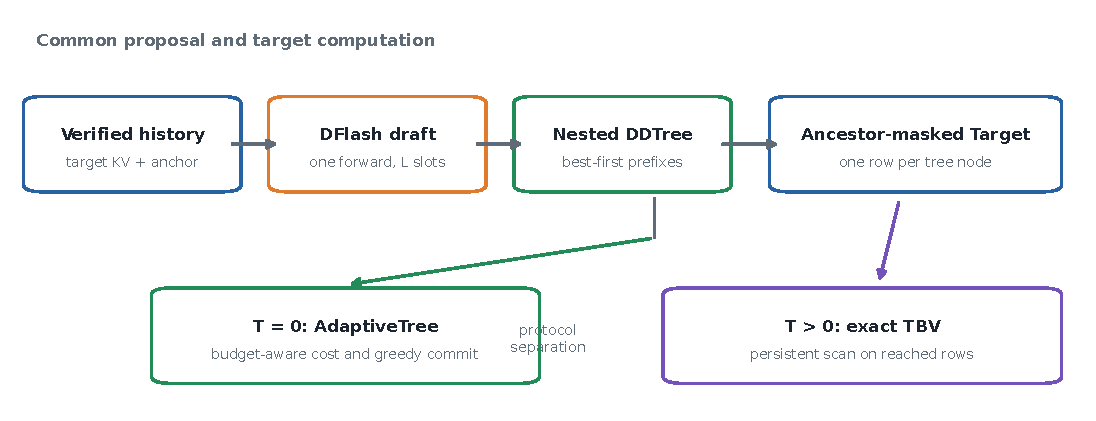
\includegraphics[width=\linewidth]{figures/system_overview.pdf}
    \caption{System overview.  A single block-diffusion forward produces $L$ position-wise distributions.  At $T=0$, \AdaptiveTree{} chooses a nested tree budget using a corrected per-budget cost model.  At $T>0$, \TBV{} and \DDTree{} receive byte-identical tree topology and FP64 target probabilities; only the post-forward verifier changes.}
    \label{fig:overview}
\end{figure}

\section{Related Work}

\paragraph{Speculative decoding.}
Independent formulations of speculative decoding established exact distribution preservation for a draft-and-correct pipeline \citep{leviathan2023fast,chen2023accelerating}.  Medusa \citep{cai2024medusa} and EAGLE-family systems \citep{li2024eagle2} use multiple heads or feature-space drafting to expose tree-shaped candidates.  Block Verification jointly couples a single draft chain to target rows and proves an optimal expected emission length for its setting \citep{sun2024block}.  Our \TBV{} problem is different: the proposal tree and target rows are frozen to \DDTree, and the accepted-prefix law is unchanged.

\paragraph{Adaptive trees and block diffusion.}
OPT-Tree optimizes draft-tree structure under a node budget \citep{wang2025opttree}.  \DDTree{} adapts best-first tree construction to position-wise distributions emitted by one block-diffusion forward \citep{ringel2026ddtree}, building on \DFlash{} \citep{chen2026dflash}.  We do not claim the best-first tree or adaptive tree construction as new.  Our deterministic component instead selects among nested \DDTree{} budgets using measured device latency, with corrected attribution of the node-dependent construction time.

\paragraph{GPU execution.}
GPU scan and reduction primitives make it possible to express a vocabulary-wide categorical draw without a sequence of host decisions.  The proposed verifier keeps one CUDA block resident across tree depths, performs a chunked FP64 reduction and exclusive scan on the current row, and traverses the sparse tree on device.  Unlike methods that alter the proposal-target coupling, this is an execution substitution for the same ancestral target sampler.

\section{Problem Setup and Architecture}
\label{sec:setup}

Let $h\in\V^*$ be the verified history and let the target model define
\begin{equation}
  p_h(x;T)=\frac{\exp(z_\theta(x\mid h)/T)}
  {\sum_{a\in\V}\exp(z_\theta(a\mid h)/T)},\qquad T>0.
  \label{eq:target}
\end{equation}
All stochastic results below hold for every fixed finite $T>0$; $T=1$ is only the registered experimental instance.  At $T=0$, $p_h$ is instead replaced by the implementation's deterministic argmax with a fixed tie rule.  One \DFlash{} forward produces logits for $L$ future slots.  For tree construction, they induce position-wise proposal distributions $q_d$ and prefix weights
\begin{equation}
  Q(u_1\ldots u_k)=\prod_{d=1}^{k}q_d(u_d),\qquad 1\leq k\leq L.
  \label{eq:draftprefix}
\end{equation}
This factorization is a proposal surrogate; it is not assumed to equal the target's autoregressive joint distribution.

\subsection{Probability trees and a single target forward}

A finite probability tree is a prefix-closed rooted tree $\T=(V,E)$ with root $\rho$.  Every non-root node $v$ has parent $\parn(v)$ and edge label $a(v)\in\V$; labels are unique among siblings.  The token prefix along the root-to-$v$ path is $s(v)$ and its depth is $|s(v)|$.  The candidate set at $v$ is
$\C(v)=\{a(w):\parn(w)=v\}$.

The root represents history $h$.  All non-root tokens are flattened into one sequence, assigned their path-consistent absolute positions, and evaluated with the mask
\begin{equation}
M_{uv}=\begin{cases}
0,&u\text{ is in the old prefix or }u\preceq v,\\
-\infty,&\text{otherwise},
\end{cases}
\label{eq:mask}
\end{equation}
where $u\preceq v$ means that $u$ is an ancestor of $v$.  Thus each row attends to the old prefix and exactly its own ancestors, never to a sibling.  Under the standard path-local transformer assumption stated in Appendix~\ref{app:treeforward}, the row at node $v$ equals the sequential conditional
\begin{equation}
  p_v(x) \equiv p_\theta(x\mid h\Vert s(v);T).
  \label{eq:nodeconditional}
\end{equation}

\subsection{Corrected \AdaptiveTree{} at \texorpdfstring{$T=0$}{T=0}}

The \DDTree{} best-first heap enumerates non-root nodes in non-increasing $Q(u)$.  Its first $b$ nodes form a valid nested tree $\T_b$.  The proposal-mass proxy
\begin{equation}
  M_b=\sum_{u\in\T_b}Q(u)
  \label{eq:massproxy}
\end{equation}
equals the expected covered prefix length under the factorized draft surrogate (Appendix~\ref{app:adaptiveproof}).  \AdaptiveTree{} enumerates once to $B_{\max}=256$ and selects from
\begin{equation}
\mathcal{B}=\{30,45,60,80,100,128,160,192,256\}.
\end{equation}
After one warm-up observation per budget, it chooses
\begin{equation}
 b_t\in\arg\max_{b\in\mathcal B}
 \frac{1+\min\{L,\widehat{s}_t M_b\}}
 {\widehat D_t+\widehat G_t(b)+\widehat V_t(b)+\widehat K_t(b)},
 \label{eq:controller}
\end{equation}
with smaller $b$ breaking ties.  Here $D$ is block-draft time, $G$ is tree construction, $V$ includes tree compilation and target verification, and $K$ is commit/cache time.  All estimates are exponential moving averages with coefficient $0.2$, and $\widehat s_t\in[0,2]$ calibrates proposal mass to observed accepted draft tokens.  The correction relative to the historical controller is the placement of $G_t(b)$ in the budget-specific denominator: constructing more nodes is not a fixed cost.  The canonical method performs no scheduled exploration after warm-up.  Budget choice changes efficiency but not the greedy acceptance rule; Appendix~\ref{app:greedy} states the deterministic equivalence result.

\subsection{Tree-block verification at \texorpdfstring{$T>0$}{T>0}}

\TBV{} receives the same $\T$ and $\{p_v\}_{v\in V}$ as \DDTree.  It draws independent uniforms $U_0,\ldots,U_D\sim\mathrm{Unif}[0,1)$, with $D$ the tree depth.  Starting at $v_0=\rho$, it samples
\begin{equation}
X_d=F_{v_d}^{-1}(U_d),\quad
F_v^{-1}(u)=\min\left\{x:\sum_{a\le x}p_v(a)>u\sum_a p_v(a)\right\}.
\label{eq:inversecdf}
\end{equation}
If $X_d\in\C(v_d)$, the unique matching child is accepted and traversal continues.  Otherwise, $X_d$ is the bonus token and the round ends.  A leaf necessarily ends the round.  Figure~\ref{fig:walk} illustrates this first-exit view.

\begin{figure}[t]
    \centering
    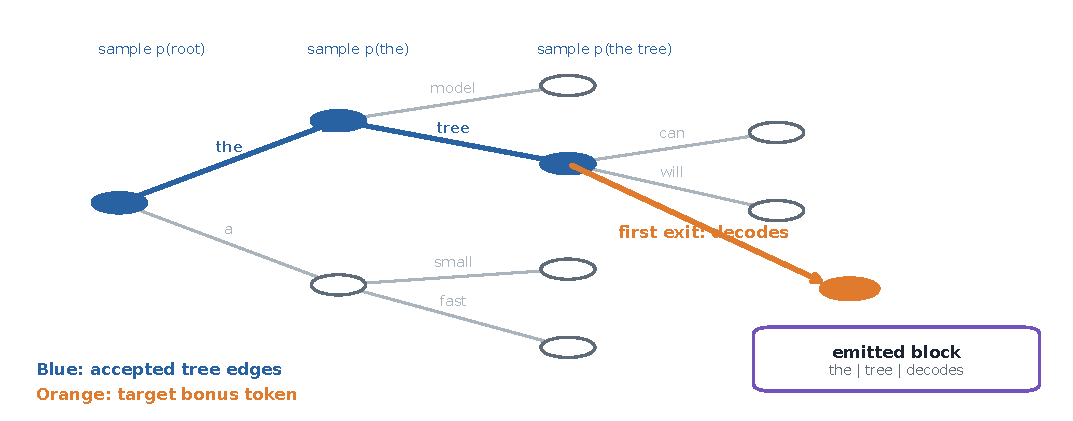
\includegraphics[width=.97\linewidth]{figures/tree_block_walk.pdf}
    \caption{One \TBV{} round.  Blue edges are sampled target tokens that match verified children; the orange edge is the first sampled token outside the tree and becomes the bonus.  The emitted block is the accepted root-to-node prefix followed by that bonus.}
    \label{fig:walk}
\end{figure}

\begin{figure}[t]
    \centering
    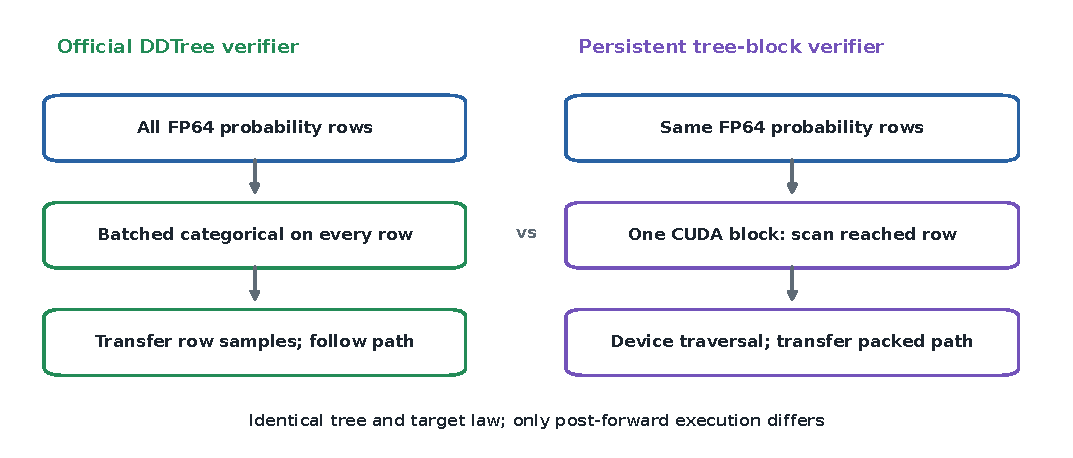
\includegraphics[width=.97\linewidth]{figures/kernel_comparison.pdf}
    \caption{Post-forward execution.  Official \DDTree{} samples all $|V|$ probability rows in one batched categorical and follows the path after a host transfer.  \TBV{} precomputes the same FP64 rows, then one persistent CUDA block scans only reached rows and returns one packed path.  Acceptance is identical in distribution on a frozen tree.}
    \label{fig:kernel}
\end{figure}

\section{Exactness of Tree-Block Verification}
\label{sec:exactness}

We give the core derivation here and a filtration-level proof in Appendix~\ref{app:fullproof}.  For $v\in V$, define the target probability of its tree prefix
\begin{equation}
\pi(v)=\prod_{(u\to w)\in\mathrm{path}(\rho,v)}p_u(a(w)),
\qquad \pi(\rho)=1,
\label{eq:prefixmass}
\end{equation}
and its exit mass
\begin{equation}
e(v)=\sum_{x\notin\C(v)}p_v(x)=1-\sum_{x\in\C(v)}p_v(x).
\label{eq:exitmass}
\end{equation}
The registered ancestral kernel never needs to materialize $e(v)$.  When terminal-mass checks are used for validation, uncovered probability is summed directly rather than obtained by subtraction, which could erase a small positive tail; the final equality in \eqref{eq:exitmass} is a real-arithmetic identity.

\begin{theorem}[Complete block law for arbitrary $T>0$]
\label{thm:blocklaw}
Fix $h$, a valid finite tree $\T$, and exact path-local rows $p_v$.  For every node $v$ and token $x\notin\C(v)$, the probability that \TBV{} emits $s(v)\Vert x$ is
\begin{equation}
  \Prb\{Z=s(v)\Vert x\mid h,\T\}=\pi(v)p_v(x).
  \label{eq:blocklaw}
\end{equation}
The events in \eqref{eq:blocklaw} are disjoint and sum to one.
\end{theorem}

\begin{proof}
The event requires sampling each edge label on the unique path to $v$, followed by $x$ at $v$.  The uniforms are independent, and inverse-CDF sampling returns row $p_u$, so multiplying the conditional factors gives $\pi(v)p_v(x)$.  Sibling-label uniqueness makes the path unique.  Every target continuation has a unique first token that is not a child of its current tree node; a finite tree guarantees this occurs no later than a leaf.  Hence these first-exit events partition the target sample space.  Equivalently,
\begin{equation}
\sum_{v\in V}\pi(v)e(v)=1,
\end{equation}
which follows by recursively splitting each prefix mass into child-prefix masses and exit mass.
\end{proof}

\begin{theorem}[Adaptive, multi-round target-law preservation for arbitrary $T>0$]
\label{thm:multiround}
Fix any finite temperature $T>0$.  At round $t$, let the tree $\T_t$ be any finite, valid, history-adaptive random tree measurable with respect to the verified history, draft randomness, and prior runtime state, but independent of the fresh verifier uniforms conditional on that state.  If tree rows satisfy \eqref{eq:nodeconditional}, concatenating \TBV{} blocks has exactly the temperature-$T$ target autoregressive distribution.
\end{theorem}

\begin{proof}
Condition on the pre-round state and $\T_t$.  Couple \TBV{} to a serial target sampler by using the same $U_d$ at each visited context.  Both samplers emit the same token from $p_\theta(\cdot\mid h\Vert X_{<d};T)$.  The tree only determines the stopping time at which the current verified block ends; it never changes a sampled token.  The bonus is already the next serial target token, and the following round resumes from the identical history.  Induction over within-round depth and then over rounds gives equality of every finite-dimensional token distribution.  Averaging over the conditioned state and random tree preserves the equality.
\end{proof}

\begin{corollary}[Same-tree acceptance identity]
\label{cor:acceptance}
Let $A$ be the number of accepted tree edges in a round.  Then
\begin{equation}
  \E[A\mid h,\T]=\sum_{v\in V\setminus\{\rho\}}\pi(v).
  \label{eq:expectedacceptance}
\end{equation}
Consequently, \TBV{} and ancestral \DDTree{} have identical accepted-length distributions on the same tree and target rows.
\end{corollary}

\begin{proof}
For each non-root node $v$, the event that traversal reaches $v$ has probability $\pi(v)$.  Summing its indicator over all non-root nodes and applying linearity of expectation yields \eqref{eq:expectedacceptance}.  The two implementations use the same row-wise target draws and child transition rule, so their complete first-exit laws agree by Theorem~\ref{thm:blocklaw}.
\end{proof}

The corollary restricts the performance claim: a same-tree verifier cannot be faster because it accepts more tokens.  It can only reduce the time after target logits exist.  Figure~\ref{fig:kernel} makes that controlled difference explicit.

\section{Persistent Inverse-CDF Kernel}
\label{sec:kernel}

Let a reached row contain nonnegative weights $w_0,\ldots,w_{m-1}$ with total $W>0$.  The kernel partitions the vocabulary contiguously across $P=640$ threads.  Thread $j$ accumulates
$S_j=\sum_{x\in I_j}w_x$.  A block-wide exclusive scan yields $A_j=\sum_{i<j}S_i$ and $W=\sum_jS_j$.  For threshold $R=UW$, exactly one nonempty chunk satisfies
\begin{equation}
 A_j\le R<A_j+S_j.
\end{equation}
That thread scans within $I_j$ to find the first token whose local cumulative mass crosses $R-A_j$.  This is exactly the global inverse CDF in \eqref{eq:inversecdf}; the formal statement, including zero-mass chunks and boundary events, is in Appendix~\ref{app:scanproof}.

After selecting token $x$, thread zero looks up the edge $(v,x)$.  If present, the kernel updates the current node and repeats; otherwise it writes the accepted path length and bonus token.  One launch therefore covers all visited depths.  The registered method intentionally retains the common full-row pipeline: BF16 target logits are converted to FP64 probability rows before either verifier.  More aggressive direct-logit and lazy-projection variants are implementation ablations, not the main method, because they change the work boundary and did not pass the frozen selection gate.

With $A$ accepted nodes, vocabulary size $m$, and tree budget $B$, the persistent kernel performs $A+1$ row scans, each $O(m/P)$ work per thread plus a $P$-way scan, and an $O(B)$ edge lookup by one thread per depth.  It stores $O(P+D)$ shared/control state and reads no unused probability row.  The official batched sampler is highly optimized, so this complexity reduction is a hardware hypothesis rather than a theorem of wall-clock speedup.

\section{Experimental Design}
\label{sec:experiments}

The experiment is intentionally split by sampling law.  Table~\ref{tab:protocols} records the frozen scope; Figure~\ref{fig:matrix} visualizes coverage.  Results are populated only after every integrity and fairness gate passes.

\begin{table}[t]
\centering
\caption{Protocol separation.  Cross-protocol averaging is forbidden.}
\label{tab:protocols}
\small
\begin{tabular}{p{.12\linewidth}p{.36\linewidth}p{.42\linewidth}}
\toprule
Protocol & Methods & Frozen conditions \\
\midrule
$T=0$ & Target, official \DFlash, \DDTree{} $B\in\{16,32,64,128,256,512,1024\}$, \AdaptiveTree{} and controls & Qwen3-4B/8B; 10 datasets; BF16; $L=15$; Target SDPA main comparison; Draft FlashAttention 2; 2,048-token cap \\
\addlinespace
$T=1$ & Target, official \DFlash, \DDTree{} $B=45$, \TBV{} $B=45$ & Qwen3-4B/8B; 8 datasets; seeds 17/29/43; Target/Draft SDPA; FP64 sampling probabilities; $L=15$; 2,048-token cap \\
\bottomrule
\end{tabular}
\end{table}

\begin{figure}[t]
    \centering
    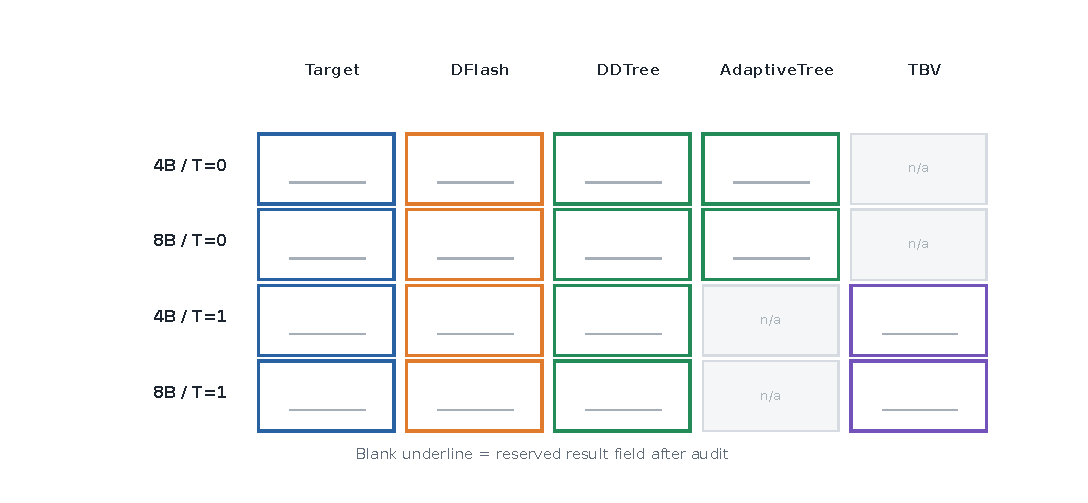
\includegraphics[width=.98\linewidth]{figures/experiment_matrix.pdf}
    \caption{Preregistered matrix.  Empty cells are intentional result slots, not missing experimental conditions.  \AdaptiveTree{} is evaluated only at $T=0$; \TBV{} only at $T=1$.}
    \label{fig:matrix}
\end{figure}

\paragraph{Datasets and models.}
The target/draft pairs are Qwen3-4B/Qwen3-4B-DFlash-b16 and Qwen3-8B/Qwen3-8B-DFlash-b16 \citep{qwen2025qwen3}, each pinned to a 40-character revision.  The $T=0$ matrix contains GSM8K \citep{cobbe2021gsm8k}, MATH-500, AIME 2024/2025, HumanEval \citep{chen2021humaneval}, MBPP-sanitized, LiveCodeBench \citep{jain2024livecodebench}, SWE-bench Lite \citep{jimenez2024swebench}, MT-Bench \citep{zheng2023mtbench}, and Alpaca.  The $T=1$ scored matrix excludes SWE-bench and Alpaca until their execution or external-judge contracts are registered.  Sampling and maximum counts follow the pinned \DDTree{} protocol.

\paragraph{Metrics.}
We report decode throughput, time per output token, speedup relative to the same-pair Target baseline, accepted draft tokens per target verification, generated length, peak memory, and task quality.  For $T=1$, every method is paired by model, dataset, source, and seed; 95\% intervals use 10,000 source-clustered bootstrap samples with all seeds for one source kept in the same cluster.  For $T=0$, the official single deterministic pass receives descriptive point estimates only.  We do not compare proposal-normalized acceptance ratios between \DFlash{} paths and \DDTree{} nodes because their denominators differ.

\paragraph{Fairness gates.}
All methods share prompts, stop rules, output caps, model revisions, and a balanced cyclic method order within each dataset.  At $T=1$, \DDTree{} and \TBV{} must emit a runtime witness showing identical parent arrays, edge tokens, complete FP64 probability-tensor hashes, generator-state hashes, and distinct executed callable hashes.  Target and Draft attention backends are identical within the $T=1$ comparison.  Objective scorers run in an identity-pinned sandbox.  A speed superiority claim is permitted only if the full 4B/8B matrix is complete and the paired 95\% confidence-interval lower bound exceeds one.

\section{Results}
\label{sec:results}

\begin{table}[t]
\centering
\caption{$T=0$ primary architecture comparison.  Speedup is relative to the paired Target-only baseline.  Every result cell is intentionally blank.}
\label{tab:t0main}
\small
\setlength{\tabcolsep}{4.0pt}
\begin{tabular}{llcccc}
\toprule
Model & Method & Speedup & TPOT (ms) & Accept/round & Exact output (\%) \\
\midrule
\multirow{4}{*}{Qwen3-4B}
 & Target & \PendingResult & \PendingResult & \PendingResult & \PendingResult \\
 & \DFlash & \PendingResult & \PendingResult & \PendingResult & \PendingResult \\
 & best fixed \DDTree & \PendingResult & \PendingResult & \PendingResult & \PendingResult \\
 & \AdaptiveTree & \PendingResult & \PendingResult & \PendingResult & \PendingResult \\
\addlinespace
\multirow{4}{*}{Qwen3-8B}
 & Target & \PendingResult & \PendingResult & \PendingResult & \PendingResult \\
 & \DFlash & \PendingResult & \PendingResult & \PendingResult & \PendingResult \\
 & best fixed \DDTree & \PendingResult & \PendingResult & \PendingResult & \PendingResult \\
 & \AdaptiveTree & \PendingResult & \PendingResult & \PendingResult & \PendingResult \\
\bottomrule
\end{tabular}
\end{table}

\begin{table}[t]
\centering
\caption{$T=1$ same-tree comparison.  Parent arrays, edge tokens, and FP64 target probability rows are required to match before these fields can be filled.  CI denotes the paired source-clustered 95\% interval.}
\label{tab:t1main}
\small
\setlength{\tabcolsep}{3.7pt}
\begin{tabular}{llcccc}
\toprule
Model & Method & Speedup vs Target & Speedup vs \DDTree & 95\% CI & Accept/round \\
\midrule
\multirow{3}{*}{Qwen3-4B}
 & \DFlash & \PendingResult & \PendingResult & \PendingWide & \PendingResult \\
 & \DDTree & \PendingResult & \PendingResult & \PendingWide & \PendingResult \\
 & \TBV & \PendingResult & \PendingResult & \PendingWide & \PendingResult \\
\addlinespace
\multirow{3}{*}{Qwen3-8B}
 & \DFlash & \PendingResult & \PendingResult & \PendingWide & \PendingResult \\
 & \DDTree & \PendingResult & \PendingResult & \PendingWide & \PendingResult \\
 & \TBV & \PendingResult & \PendingResult & \PendingWide & \PendingResult \\
\bottomrule
\end{tabular}
\end{table}

\paragraph{Current status.}
No numerical conclusion is made in this draft.  In particular, the blank cells must not be filled from pilot runs, incomplete submatrices, microbenchmarks, or runs that fail the output-quality, same-tree, environment, order-balance, coverage, or report-reconstruction gates.


\section{Discussion and Limitations}

The system deliberately makes a narrower claim than ``tree decoding is faster.''  \AdaptiveTree{} optimizes a measured throughput surrogate at $T=0$; it is neither reinforcement learning nor a proof of globally optimal latency.  \TBV{} is exact for the stochastic target law, but its same-tree accepted length is provably identical to \DDTree.  The persistent kernel may lose to a tuned batched categorical on a particular GPU, vocabulary size, or tree shape.  Such a result is a valid negative outcome, not a correctness failure.

The mathematical theorems use exact real arithmetic and path-local target rows.  The implementation uses BF16 model computation and FP64 probability arithmetic.  Floating-point reductions, finite mask sentinels, and shape-dependent attention kernels can prevent bitwise equality even when the abstract sampling law is exact.  We therefore separate distributional unit tests from real-checkpoint output audits and report any greedy BF16 mismatch rather than filtering it out.  Finally, results on two Qwen3 model sizes do not establish behavior for larger dense or mixture-of-experts models.

\section*{Reproducibility Statement}
The full algorithm, assumptions, and proofs appear in Sections~\ref{sec:setup}--\ref{sec:kernel} and Appendices~\ref{app:fullproof}--\ref{app:greedy}.  Appendix~\ref{app:protocol} lists the frozen model revisions, dataset counts, seeds, backends, precision settings, method-order policy, and audit gates.  The supplementary code contains the official-source hashes, CUDA implementation, exact finite-law tests, same-tree runtime witness, run manifests, and report rebuilders.  Result tables remain blank until a fresh run satisfies the registered completion checks.

\section*{Ethics Statement}
This work studies inference efficiency and does not train or release a new language model.  Faster generation can reduce compute cost but may also increase the scale at which model outputs are produced.  Benchmark prompts and model outputs should be handled under their source licenses and privacy terms.  We report quality alongside speed and do not treat faster generation as evidence of safer or more reliable model behavior.

\bibliography{references}
\bibliographystyle{iclr2027_conference}

\section*{AI Use Statement}
Generative AI tools were used to assist with source-code navigation, LaTeX drafting, figure scripting, and language editing.  The authors are responsible for the mathematical claims, implementation-to-equation correspondence, citations, experiment execution, and final manuscript.  No AI-generated numerical result is reported; all quantitative fields are intentionally blank pending audited experiments.

\clearpage
\appendix

\section{Complete Probability Model}
\label{app:fullproof}

\subsection{Filtration and admissible adaptive trees}

Let $Y_1,Y_2,\ldots$ denote generated tokens and let $\mathcal{F}_t$ contain the prompt, all tokens committed before round $t$, draft-model randomness, previous verifier randomness, caches, timing observations, and controller state.  The round-$t$ tree $\T_t$ is \emph{admissible} when it is finite, prefix-closed, has unique sibling labels, and is measurable with respect to $\mathcal{F}_t$ plus fresh draft randomness generated before verification.  The verifier uniforms $U_{t,0},\ldots,U_{t,D_t}$ are conditionally independent of $\T_t$ given that pre-verification state.

This condition allows the tree to depend on the full history, proposal logits, prompt class, past acceptances, past timings, and hardware state.  It forbids choosing or expanding the current tree after observing a fresh target sample from the row being verified.  The target rows themselves are deterministic functions of the model, history, and tree paths.

\subsection{Path and terminal-event derivation}

Write $v_0=\rho,v_1,\ldots,v_k=v$ for the path to $v$, and $a_i=a(v_i)$.  The event that traversal reaches $v$ is
\begin{equation}
R_v=\{X_0=a_1,\ldots,X_{k-1}=a_k\}.
\end{equation}
Conditional on the tree and history,
\begin{align}
\Prb(R_v\mid\mathcal F_t,\T_t)
&=\prod_{i=0}^{k-1}\Prb(X_i=a_{i+1}\mid X_{<i}=a_{1:i},\mathcal F_t,\T_t)\\
&=\prod_{i=0}^{k-1}p_{v_i}(a_{i+1})=\pi(v).
\end{align}
For $x\notin\C(v)$, define $E_{v,x}=R_v\cap\{X_k=x\}$.  Then
\begin{equation}
\Prb(E_{v,x}\mid\mathcal F_t,\T_t)=\pi(v)p_v(x).
\label{eq:terminaleventapp}
\end{equation}
The events $E_{v,x}$ are pairwise disjoint: two distinct outputs either diverge on a sampled token or stop at different first-exit positions.  They are exhaustive because every root-to-leaf walk reaches a node without a matching child in finite depth.  Summing \eqref{eq:terminaleventapp} yields one.

An algebraic proof uses the recursion
\begin{equation}
\pi(v)=\pi(v)e(v)+\sum_{w:\parn(w)=v}\pi(w).
\end{equation}
Applying it from the root down telescopes all internal child masses and leaves $\sum_v\pi(v)e(v)=\pi(\rho)=1$.  Conditional on exiting at $v$, the bonus token law is
\begin{equation}
\Prb(X=x\mid\text{exit at }v)=\frac{p_v(x)\mathbf 1\{x\notin\C(v)\}}{e(v)}
\end{equation}
when $e(v)>0$.  Multiplying by terminal-node mass $\pi(v)e(v)$ recovers \eqref{eq:terminaleventapp}.  This terminal-mass factorization is a proof device; the registered kernel implements the equivalent ancestral process.

\subsection{Stopping-time proof of autoregressive exactness}

Consider an infinite serial target sequence generated from independent uniforms $U_1,U_2,\ldots$ via inverse CDF at the current history.  Given an admissible tree, define
\begin{equation}
\tau=\min\{k\ge1:Y_k\notin\C(v_{k-1})\},
\end{equation}
where $v_{k-1}$ is the tree node reached by $Y_{1:k-1}$.  Because $\T$ is finite, $\tau\le D+1$.  The event $\{\tau=k\}$ is determined by $Y_{1:k}$ and the fixed tree, so $\tau$ is a bounded stopping time.  \TBV{} emits exactly $Y_{1:\tau}$.  Restarting with fresh uniforms after $\tau$ is distributionally identical to continuing the serial sampler, because the target conditional depends only on the committed history.  Repeating at successive bounded stopping times partitions, but never changes, the serial target sequence.  This proves Theorem~\ref{thm:multiround}.

\subsection{Accepted-length distribution}

For $d\ge1$, let $V_d$ be the set of depth-$d$ nodes.  Since these path events are mutually exclusive,
\begin{equation}
\Prb(A\ge d\mid h,\T)=\sum_{v\in V_d}\pi(v).
\end{equation}
The tail-sum identity gives
\begin{align}
\E[A\mid h,\T]
&=\sum_{d=1}^{D}\Prb(A\ge d\mid h,\T)\\
&=\sum_{v\in V\setminus\{\rho\}}\pi(v).
\end{align}
The entire distribution of $A$, not merely its expectation, is a function only of $\T$ and target rows.  Therefore an implementation-only verifier substitution cannot honestly claim a systematic acceptance improvement under a same-tree replay.

\section{Correctness of the Tree Target Forward}
\label{app:treeforward}

\begin{assumption}[Path locality]
The target is in deterministic evaluation mode.  For every tree node, token identity, absolute position, positional transformation, and allowed attention keys equal those of its serial root-to-node sequence.  Non-attention operations act independently per position.  Masked attention probabilities are exactly zero, and the incoming KV cache equals the serial cache for the verified history.
\end{assumption}

\begin{lemma}[Tree-row equivalence]
Under path locality, the hidden state, KV entries, and output logits at node $v$ equal those obtained by serially evaluating $h\Vert s(v)$.
\end{lemma}

\begin{proof}
Proceed by transformer layer.  At the input, the token embedding and positional representation of $v$ match serial evaluation.  Suppose all representations and cached keys/values visible to $v$ match at layer $\ell$.  Equation~\eqref{eq:mask} exposes exactly the old prefix and ancestors with identical positions, so queries, keys, values, attention normalization, and weighted sums match.  Sibling representations are masked and contribute zero.  Position-wise residual, normalization, and feed-forward operations therefore match, establishing the induction step.  The final language-model head gives the same logits, and the layer-wise keys and values match as well.
\end{proof}

In finite precision, a large negative mask sentinel is not literally $-\infty$, and different attention shapes may select different kernels.  The lemma is the exact-computation contract; real-checkpoint audits separately test token or distributional behavior.

\section{Equivalence of the Parallel Chunk Scan}
\label{app:scanproof}

Let contiguous chunks $I_0,\ldots,I_{P-1}$ partition $\{0,\ldots,m-1\}$.  Define
\begin{equation}
S_j=\sum_{x\in I_j}w_x,\quad A_j=\sum_{i<j}S_i,\quad
C(x)=\sum_{a=0}^{x}w_a.
\end{equation}

\begin{theorem}[Chunk-scan inverse-CDF equivalence]
For $w_x\ge0$, $W=\sum_xw_x>0$, and $U\sim\mathrm{Unif}[0,1)$, the two-stage rule
\begin{enumerate}[leftmargin=1.4em,itemsep=1pt]
\item choose the unique chunk $j$ satisfying $A_j\le UW<A_j+S_j$;
\item return the smallest $x\in I_j$ satisfying $C(x)>UW$
\end{enumerate}
returns token $x$ with probability $w_x/W$ and agrees almost surely with a global inverse-CDF draw.
\end{theorem}

\begin{proof}
Zero-mass chunks contain no threshold interval and cannot be selected.  For every positive-mass chunk, $[A_j,A_j+S_j)$ is exactly the disjoint interval covered by its tokens.  Within the selected chunk, subtracting the exclusive prefix $A_j$ leaves the same ordered cumulative token intervals as the global CDF.  Thus token $x$ is returned exactly when
\begin{equation}
C(x-1)\le UW<C(x),
\end{equation}
with $C(-1)=0$.  This interval has length $w_x$, so its probability under uniform $UW$ on $[0,W)$ is $w_x/W$.  Threshold equality at an internal boundary has probability zero for an ideal continuous uniform; the implementation fixes a strict comparison rule for reproducibility.
\end{proof}

The CUDA kernel applies this theorem at the current node, then performs a deterministic child lookup.  Conditional on reaching the next node, the next independent uniform invokes the theorem again.  Induction over depth yields the same path as serial inverse-CDF ancestral sampling for the supplied uniform vector.

\section{Adaptive Budget Properties at \texorpdfstring{$T=0$}{T=0}}
\label{app:adaptiveproof}

For a prefix-closed tree $\T$ and an auxiliary draft sequence $X_{1:L}\sim\prod_dq_d$, define its covered prefix length
\begin{equation}
A_{\T}(X)=\max\bigl(\{0\}\cup\{d:X_{1:d}\in\T\}\bigr).
\end{equation}

\begin{proposition}[Mass proxy identity]
For every finite prefix-closed $\T$,
\begin{equation}
\E_Q[A_\T(X)]=\sum_{u\in\T}Q(u).
\end{equation}
\end{proposition}

\begin{proof}
Prefix closure implies $\{A_\T\ge d\}=\{X_{1:d}\in\T\}$.  Using the tail-sum formula and disjoint depth-$d$ prefixes,
\begin{equation}
\E_Q[A_\T]=\sum_{d=1}^{L}\sum_{u\in\T:|u|=d}Q(u)=\sum_{u\in\T}Q(u).
\end{equation}
\end{proof}

The best-first \DDTree{} predecessor rule guarantees that a node enters the heap only after its parent or preceding sibling.  Since both parent and preceding sibling have no smaller weight, the heap frontier always contains a predecessor of every unenumerated candidate.  Therefore the next pop is a maximum-weight remaining node, every enumeration prefix is prefix-closed, and $\T_b$ maximizes the proxy mass among size-$b$ trees in the retained candidate space.  This is a property of \DDTree, not a new optimality claim for the latency controller.  Equation~\eqref{eq:controller} uses this proxy only as one input; it does not imply global throughput optimality.

\section{Greedy Output Equivalence}
\label{app:greedy}

At $T=0$, let $g(c)$ be the target argmax under the fixed tie rule.  Starting from verified context $c$, the tree verifier queries the root row.  If $g(c)$ labels a child, it accepts that child and repeats at the corresponding path-local row.  Otherwise it emits $g(c)$ as bonus.  By induction, every accepted node and the bonus equal the next tokens of serial greedy decoding.  The selected budget may depend arbitrarily on the current proposal, prior timings, acceptance history, and controller state, because correctness holds for every valid tree.  Cache compaction retains the root and accepted path KV entries but not the bonus, which becomes the next round's anchor.  A second induction over rounds proves equality to serial greedy decoding under the same EOS and length rules, subject to the exact path-locality assumption.

\section{Full Experimental Contract}
\label{app:protocol}

\begin{table}[h]
\centering
\caption{Frozen model identities.}
\small
\begin{tabular}{lll}
\toprule
Role & Qwen3-4B pair & Qwen3-8B pair \\
\midrule
Target revision & \texttt{1cfa9a720891...b3df60c} & \texttt{b968826d9c46...de91218} \\
Draft revision & \texttt{b74e3a329c4d...2be72bd} & \texttt{9b41424b7109...85333f4} \\
Weights & BF16 & BF16 \\
Thinking & disabled & disabled \\
\bottomrule
\end{tabular}
\end{table}

\begin{table}[h]
\centering
\caption{Frozen dataset counts per model.  MT-Bench contains two turns and therefore more generation calls than source rows.}
\small
\begin{tabular}{lrrrrrrrrrr}
\toprule
 & GSM8K & MATH & A24 & A25 & HE & MBPP & LCB & SWE & MT & Alpaca \\
\midrule
$T=0$ & 128 & 128 & 30 & 30 & 164 & 128 & 128 & 128 & 80 & 128 \\
$T=1$ & 128 & 128 & 30 & 30 & 164 & 128 & 128 & -- & 80 & -- \\
\bottomrule
\end{tabular}
\end{table}

The $T=0$ primary table compares all architectures under Target SDPA and Draft FlashAttention 2.  A Target-FA2 Target/\DFlash{} run is auxiliary and is never silently mixed with tree methods.  The method schedule is a deterministic cyclic rotation whose per-dataset position-count imbalance is at most one.  The canonical \AdaptiveTree{} candidate set is $\{30,45,60,80,100,128,160,192,256\}$, with a one-observation warm-up per budget, EWMA coefficient $0.2$, and no periodic exploration.

At $T=1$, both Target and Draft use SDPA, $L=15$, $B=45$, and FP64 probabilities.  \DFlash{} retains its official greedy draft proposal, while \DDTree{} and \TBV{} use draft temperature 1.  Seeds are 17, 29, and 43.  Every completed record must bind the run identifier, model and data manifests, method order, source identifier, seed, prompt hash, output hash, timing, generated length, accepted length, and scorer result.  The report is rebuilt from raw JSONL records rather than trusting cached tables.

\section{Additional Blank Result Tables}
\label{app:blanktables}

\begin{table}[h]
\centering
\caption{Per-dataset $T=0$ speedup relative to Target.}
\small
\setlength{\tabcolsep}{3.0pt}
\resizebox{\textwidth}{!}{%
\begin{tabular}{llrrrrrrrrrr}
\toprule
Model & Method & GSM8K & MATH & A24 & A25 & HE & MBPP & LCB & SWE & MT & Alpaca \\
\midrule
Qwen3-4B & \DFlash & \PendingResult&\PendingResult&\PendingResult&\PendingResult&\PendingResult&\PendingResult&\PendingResult&\PendingResult&\PendingResult&\PendingResult\\
 & best \DDTree & \PendingResult&\PendingResult&\PendingResult&\PendingResult&\PendingResult&\PendingResult&\PendingResult&\PendingResult&\PendingResult&\PendingResult\\
 & \AdaptiveTree & \PendingResult&\PendingResult&\PendingResult&\PendingResult&\PendingResult&\PendingResult&\PendingResult&\PendingResult&\PendingResult&\PendingResult\\
\addlinespace
Qwen3-8B & \DFlash & \PendingResult&\PendingResult&\PendingResult&\PendingResult&\PendingResult&\PendingResult&\PendingResult&\PendingResult&\PendingResult&\PendingResult\\
 & best \DDTree & \PendingResult&\PendingResult&\PendingResult&\PendingResult&\PendingResult&\PendingResult&\PendingResult&\PendingResult&\PendingResult&\PendingResult\\
 & \AdaptiveTree & \PendingResult&\PendingResult&\PendingResult&\PendingResult&\PendingResult&\PendingResult&\PendingResult&\PendingResult&\PendingResult&\PendingResult\\
\bottomrule
\end{tabular}}
\end{table}

\begin{table}[h]
\centering
\caption{Per-dataset $T=1$ throughput speedup.  The first value is versus Target; the parenthesized value is versus \DDTree.}
\small
\setlength{\tabcolsep}{3.2pt}
\resizebox{\textwidth}{!}{%
\begin{tabular}{llrrrrrrrr}
\toprule
Model & Method & GSM8K & MATH & A24 & A25 & HE & MBPP & LCB & MT \\
\midrule
Qwen3-4B & \DFlash & \PendingWide&\PendingWide&\PendingWide&\PendingWide&\PendingWide&\PendingWide&\PendingWide&\PendingWide\\
 & \DDTree & \PendingWide&\PendingWide&\PendingWide&\PendingWide&\PendingWide&\PendingWide&\PendingWide&\PendingWide\\
 & \TBV & \PendingWide&\PendingWide&\PendingWide&\PendingWide&\PendingWide&\PendingWide&\PendingWide&\PendingWide\\
\addlinespace
Qwen3-8B & \DFlash & \PendingWide&\PendingWide&\PendingWide&\PendingWide&\PendingWide&\PendingWide&\PendingWide&\PendingWide\\
 & \DDTree & \PendingWide&\PendingWide&\PendingWide&\PendingWide&\PendingWide&\PendingWide&\PendingWide&\PendingWide\\
 & \TBV & \PendingWide&\PendingWide&\PendingWide&\PendingWide&\PendingWide&\PendingWide&\PendingWide&\PendingWide\\
\bottomrule
\end{tabular}}
\end{table}

\begin{table}[h]
\centering
\caption{AdaptiveTree ablations at $T=0$.  Values are geometric-mean speedups relative to the paired Target baseline.}
\small
\setlength{\tabcolsep}{4.0pt}
\begin{tabular}{lccp{.46\linewidth}}
\toprule
Variant & Qwen3-4B & Qwen3-8B & Single changed factor \\
\midrule
\AdaptiveTree & \PendingResult & \PendingResult & canonical controller \\
$B\le128$ & \PendingResult & \PendingResult & remove 160/192/256 candidates \\
legacy cost attribution & \PendingResult & \PendingResult & treat tree build as fixed proposal cost \\
with periodic exploration & \PendingResult & \PendingResult & restore one forced probe every 64 decisions \\
no acceptance calibration & \PendingResult & \PendingResult & fix $\widehat s_t=1$ \\
no measured latency & \PendingResult & \PendingResult & rank budgets by calibrated proposal mass only \\
frozen after warm-up & \PendingResult & \PendingResult & disable subsequent EWMA updates \\
historical controller & \PendingResult & \PendingResult & old budget, attribution, and exploration package \\
\bottomrule
\end{tabular}
\end{table}

\begin{table}[h]
\centering
\caption{Verifier-only same-state replay.  Latency ratios are \DDTree{} verifier time divided by candidate verifier time.}
\small
\begin{tabular}{lcccc}
\toprule
Model & $T=1$ ratio & Kernel time ($\mu$s) & Peak memory (MiB) & Law test \\
\midrule
Qwen3-4B & \PendingResult & \PendingResult & \PendingResult & \PendingResult \\
Qwen3-8B & \PendingResult & \PendingResult & \PendingResult & \PendingResult \\
\bottomrule
\end{tabular}
\end{table}

\begin{table}[h]
\centering
\caption{Task-quality audit at $T=1$.  MT-Bench requires a separately registered external judge and is shown as not scored here.}
\small
\begin{tabular}{llcccc}
\toprule
Model & Method & Math accuracy & Code pass rate & Mean gen. length & MT-Bench \\
\midrule
Qwen3-4B & Target & \PendingResult & \PendingResult & \PendingResult & -- \\
 & \DFlash & \PendingResult & \PendingResult & \PendingResult & -- \\
 & \DDTree & \PendingResult & \PendingResult & \PendingResult & -- \\
 & \TBV & \PendingResult & \PendingResult & \PendingResult & -- \\
\addlinespace
Qwen3-8B & Target & \PendingResult & \PendingResult & \PendingResult & -- \\
 & \DFlash & \PendingResult & \PendingResult & \PendingResult & -- \\
 & \DDTree & \PendingResult & \PendingResult & \PendingResult & -- \\
 & \TBV & \PendingResult & \PendingResult & \PendingResult & -- \\
\bottomrule
\end{tabular}
\end{table}


\end{document}
